\documentclass[]{article}
\usepackage{lmodern}
\usepackage{amssymb,amsmath}
\usepackage{ifxetex,ifluatex}
\usepackage{fixltx2e} % provides \textsubscript
\ifnum 0\ifxetex 1\fi\ifluatex 1\fi=0 % if pdftex
  \usepackage[T1]{fontenc}
  \usepackage[utf8]{inputenc}
\else % if luatex or xelatex
  \ifxetex
    \usepackage{mathspec}
  \else
    \usepackage{fontspec}
  \fi
  \defaultfontfeatures{Ligatures=TeX,Scale=MatchLowercase}
\fi
% use upquote if available, for straight quotes in verbatim environments
\IfFileExists{upquote.sty}{\usepackage{upquote}}{}
% use microtype if available
\IfFileExists{microtype.sty}{%
\usepackage{microtype}
\UseMicrotypeSet[protrusion]{basicmath} % disable protrusion for tt fonts
}{}
\usepackage[unicode=true]{hyperref}
\hypersetup{
            pdfborder={0 0 0},
            breaklinks=true}
\urlstyle{same}  % don't use monospace font for urls
\usepackage{graphicx,grffile}
\makeatletter
\def\maxwidth{\ifdim\Gin@nat@width>\linewidth\linewidth\else\Gin@nat@width\fi}
\def\maxheight{\ifdim\Gin@nat@height>\textheight\textheight\else\Gin@nat@height\fi}
\makeatother
% Scale images if necessary, so that they will not overflow the page
% margins by default, and it is still possible to overwrite the defaults
% using explicit options in \includegraphics[width, height, ...]{}
\setkeys{Gin}{width=\maxwidth,height=\maxheight,keepaspectratio}
\IfFileExists{parskip.sty}{%
\usepackage{parskip}
}{% else
\setlength{\parindent}{0pt}
\setlength{\parskip}{6pt plus 2pt minus 1pt}
}
\setlength{\emergencystretch}{3em}  % prevent overfull lines
\providecommand{\tightlist}{%
  \setlength{\itemsep}{0pt}\setlength{\parskip}{0pt}}
\setcounter{secnumdepth}{0}
% Redefines (sub)paragraphs to behave more like sections
\ifx\paragraph\undefined\else
\let\oldparagraph\paragraph
\renewcommand{\paragraph}[1]{\oldparagraph{#1}\mbox{}}
\fi
\ifx\subparagraph\undefined\else
\let\oldsubparagraph\subparagraph
\renewcommand{\subparagraph}[1]{\oldsubparagraph{#1}\mbox{}}
\fi

% set default figure placement to htbp
\makeatletter
\def\fps@figure{htbp}
\makeatother


\date{}

\begin{document}

Igiene Medicina Generale 25 01 2017

dott. Del Canale

Sbobinatore Stefania Manno

EMPATIA MEDICO -- PAZIENTE (sezione)

DEFINIZIONE DI EMPATIA (sottosezione)

L'empatia medico - paziente è alla base della professione, qualsiasi sia
la specialità.

\emph{``L'essere sani è in realtà l'ignoranza di essere malati''}

da ``Dr Knock, o il trionfo della medicina''

Si tratta di una commedia francese (1923) che canzona l'onnipotenza
della classe medica del tempo. In sintesi: la commedia è ambientata nel
paese di Sant Maurice, i protagonisti sono due medici, il dott.
Parpalaid e il dott. Knock. Il dott. Parpalaid è un medico empatico,
suggerisce ai pazienti di seguire uno stile di vita sano, senza
medicalizzare la questione, senza toni paternalistici (``il clima
salubre di Sant Maurice è il migliore alleato del medico''). Risultato:
in paese tutti sono sani. Il medico si trasferisce a Lione e viene
sostituito dal dott. Knock che invece ha l'intenzione di mercificare la
medicina per ottenere facili guadagni. Risultato: in breve tempo il
paese diventa un paese di malati.

I concetti che questa commedia permette di introdurre sono:

\begin{itemize}
\item
  \textbf{disease mongering} ovvero commercializzazione, mercificazione
  della medicina;
\item
  creazione di \textbf{pre-patologie} (pre-diabete, ipertensione
  normale-alta, riduzione valori soglia di colesterolo) ovvero la
  tendenza a ridurre i valori soglia tanto da definire tutta la
  popolazione malata;
\item
  \textbf{tecnologia} che oscilla fra un reale supporto al progresso
  della medicina e il supporto alle false patologie.
\end{itemize}

\emph{``Tutti siamo stati creati per sentire empatia verso i nostri
simili.''}

da Homo Empaticus di Jeremy Rifkin

L'empatia salverà il mondo, le relazioni umane.

\emph{``All'empatia serve un progetto, solo così genera condivisione''}

da Un mondo condiviso di Laura Boella

Libro a cui ha partecipato Rizzolatti la cui teoria dei neuroni specchio
costituisce la base razionale dell'empatia. L'empatia non deve essere
astratta ma necessita di un progetto, solo così genera condivisione:

\begin{enumerate}
\def\labelenumi{\arabic{enumi}.}
\item
  il medico è un mestiere di relazione
\item
  il ruolo di medico non è sufficiente per avere credibilità
\item
  è necessaria una co-costruzione della relazione medico-paziente, l'uno
  ha bisogno dell'altro per raggiungere degli obiettivi.
\end{enumerate}

Hojat (Jefferson University) definisce l'empatia come \emph{qualità
prevalentemente cognitiva} (piuttosto che emozionale) che si basa su una
\emph{conoscenza} (piuttosto che su una sensazione) delle esperienze,
dei timori e della visione del paziente combinata con la \emph{capacità
di comunicare} questa conoscenza e con \emph{l'intenzione di aiutare il
paziente stesso}.

Altre definizioni di empatia nel contesto della cura:

\begin{itemize}
\item
  attitudine innata o acquisita che favorisce il rapporto tra figura
  sanitaria e paziente;
\item
  requisito sufficiente per raggiungere obiettivi di salute dimostrabili
  scientificamente. Questa definizione è una novità, la novità sta nel
  fatto che all'empatia si associano risultati clinici significativi.
\end{itemize}

Luigi Ripamonti (responsabile del Corriere Salute), editoriale ``Medici
empatici e Anti-empatici'': ``{[}\ldots{}{]} le prime qualità da
ricercare in professionisti nelle mani dei quali si mette la propria
salute, in un periodo in cui la medicina viene sempre più percepita,
dagli stessi medici, come fin troppo pervasa da algidi algoritmi,
tecnologia e obblighi amministrativi {[}\ldots{}{]} l'importanza di
stabilire una sintonia emotiva con i pazienti dovrebbe essere riscoperta
e valorizzata, anche per rivendicare alla professione medica la sua
titolarità di arte {[}\ldots{}{]}''

La percezione del paziente dell'empatia del medico è significativamente
correlata:

\begin{itemize}
\item
  alla soddisfazione dell'operato del medico stesso;
\item
  alla compliance del paziente.
\end{itemize}

EMPATIA ED ADERENZA TERAPEUTICA (sottosezione)

Applicazione dell'empatia medico -- paziente è il raggiungimento
dell'aderenza terapeutica. Il paziente non necessariamente si attiene a
quanto indicato dal medico, l'aderenza terapeutica è difficile da
raggiungere.

\emph{``I farmaci non funzionano nei pazienti che non li assumo.''}

C. Everett Koop

\emph{``Date un'occhiata agli errori dei pazienti, perché spesso mentono
riguardo ai farmaci prescritti. Per non assumere bevande di cattivo
gusto o purgative essi talora muoiono.''}

Ippocrate

Il termine \textbf{compliance}, preferito fino alla fine degli anni `90,
implica un'asimmetria decisionale tra medico, che pone indicazioni al
trattamento, e paziente, che deve attenersi alla prescrizioni. È una
relazione rigida: il medico prescrive il trattamento e il paziente si
deve attenere.

Il termine \textbf{aderenza} invece è più corretto e privo di
correlazioni paternaliste in quanto sottolinea il ruolo attivo del
paziente e la sua partecipazione al trattamento.

Il termine da utilizzare al giorno d'oggi è \textbf{concordanza}, basato
sul concetto che l'alleanza terapeutica tra medico e paziente è un
processo di negoziazione, che nasce nel rispetto delle esigenze di
entrambi (connotato di una medicina evoluta). Questo non significa che
il medico si debba spogliare della sua autorevolezza e della sua scienza
ma che non può confidare solo nell'autorevolezza e nella scienza per far
comprendere al paziente la necessità di una terapia piuttosto che di
un'altra.

STUDI CLINICI (sotto-sottosezione)

INTERRUZIONE DELLA TERAPIA CON STATINE NEL CONTESTO DELLA PREVENZIONE
PRIMARIA O SECONDARIA DELLA CARDIOPATIA ISCHEMICA (paragrafo)

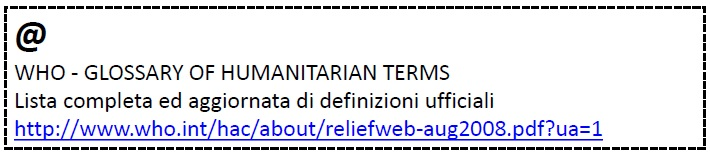
\includegraphics[width=5.96675in,height=3.55208in]{media/image1.jpeg}

A due anni dall'inizio della terapia con statine, la percentuale di
pazienti che continua ad assumere la terapia è: 1) del 40\% nei pazienti
con storia recente di SCA, 2) del 30\% nei pazienti con cardiopatia
ischemica cronica, 3) del 25\% nei pazienti che assumono statine come
prevenzione primaria.

I fattori predittivi (che permettono di presagire) di interruzione della
terapia con statine:

\begin{itemize}
\item
  età avanzata \textgreater{} 75 anni
\item
  basso livello socio economico
\item
  depressione o demenza
\item
  terapia con più di 10 farmaci (politerapia, perché il paziente non sa
  quale sia il suo farmaco più importante)
\item
  assenza di eventi acuti negli ultimi 12 mesi (``perché prendere il
  farmaco se non è successo nulla?'').
\end{itemize}

INTERRUZIONE DELLA TERAPIA CON STATINE DOPO ICTUS ISCHEMICO (Paragrafo)

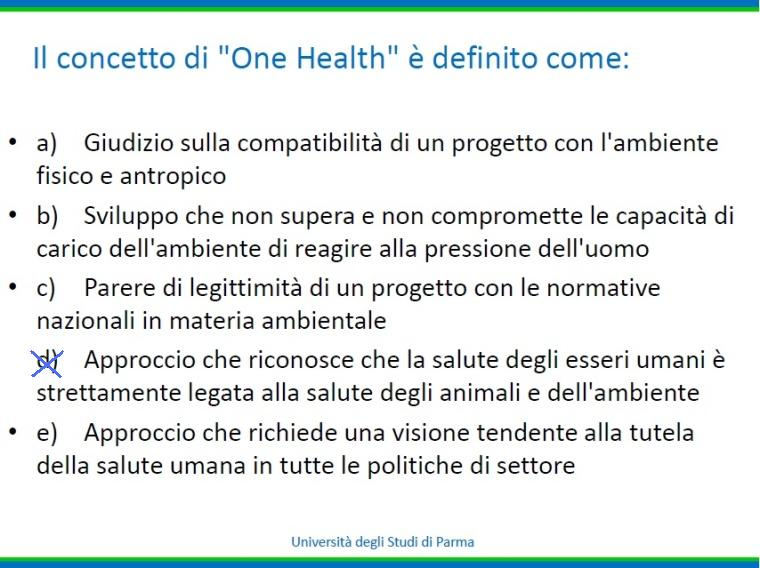
\includegraphics[width=5.41023in,height=3.34340in]{media/image2.jpeg}

A 12 mesi dall'ictus il 50\% dei pazienti ha sospeso la statina,
trattamento dato a scopo di prevenzione secondaria.

I fattori predittivi di interruzione della terapia con statine sono:

\begin{itemize}
\item
  età avanzata \textgreater{} 75 anni;
\item
  depressione post-ictale
\item
  sesso femminile
\item
  assenza di diabete mellito
\end{itemize}

IMPATTO DELL'INTERRUZIONE DELLE ``EVIDENCE -- BASED MEDICAL THERAPIES''
SULLA PROGNOSI CLINICA DOPO INFARTO MIOCARDICO ACUTO (paragrafo)

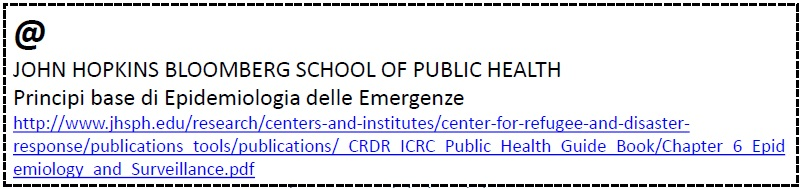
\includegraphics[width=4.57292in,height=2.45794in]{media/image3.jpeg}

Dati dal Registro Premier, tenuto dai medici di medicina generale in
Scozia. Secondo la EBM, a meno che non vi siano allergie, nel paziente
infartuato devono essere somministrati aspirina, beta bloccanti, ACE
(non rientrano nello studio) e statine. L'interruzione della terapia con
aspirina comporta un raddoppio della mortalità, l'interruzione dei beta
bloccanti comporta anch'essa una mortalità doppia, l'interruzione della
terapia con statine comporta un triplarsi della mortalità.

CAUSE DI INTERRUZIONE DELLA TERAPIA CON STATINE (paragrafo)

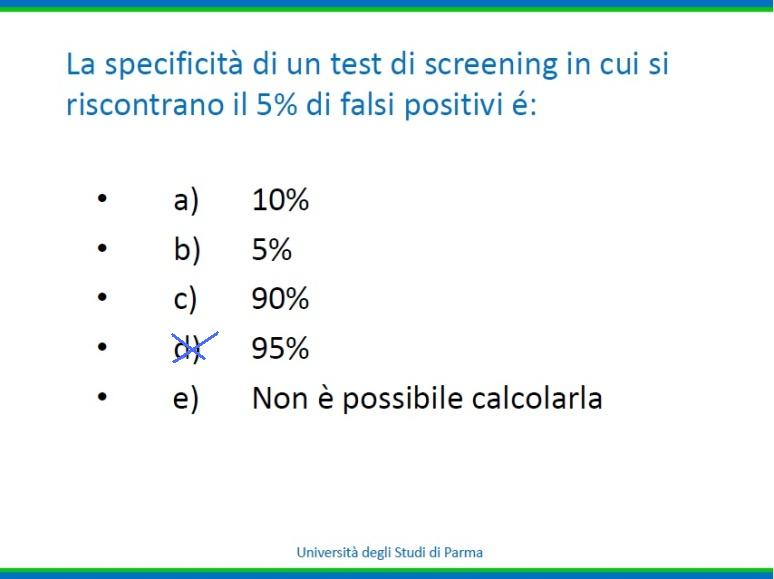
\includegraphics[width=4.69792in,height=2.68884in]{media/image4.jpeg}

Le cause di interruzione di terapia con statine sono:

\begin{itemize}
\item
  nel 72\% dei casi, in assenza di evidenti motivi clinici, il paziente
  riferisce di aver sospeso la terapia perché assume ``troppe
  pastiglie'';
\item
  nel 28\% dei casi la terapia viene sospesa perché insorgono lievi
  effetti collaterali (dispepsia, astenia, cefalea, mialgie). Sono le
  mialgie (11\% del 28\%, 2\% dei pazienti) l'effetto collaterale che
  più spesso obbliga a sospendere la terapia.
\end{itemize}

FATTORI DEMOGRAFICI, CLINICI E SOCIO ECONOMICI POTENZIALMENTE PREDITTIVI
DI MANCATA ADERENZA (sotto-sottosezione)

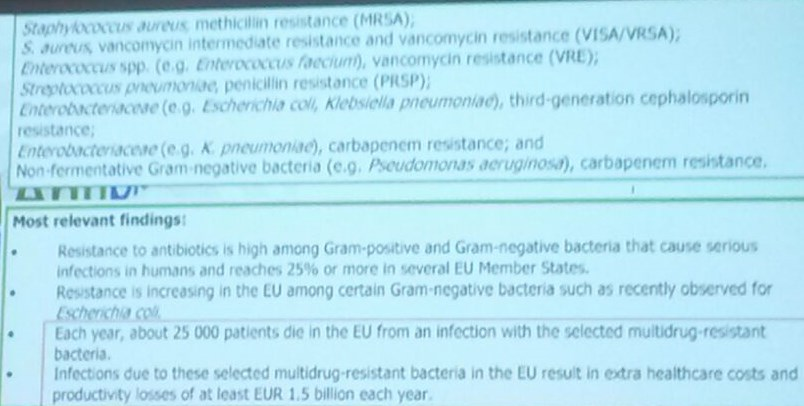
\includegraphics[width=5.86687in,height=2.66933in]{media/image5.jpeg}

Condizioni asintomatiche: il paziente asintomatico aderisce meno alla
terapia rispetto al paziente sintomatico, quest'ultimo assume la terapia
perché crede che l'aiuti, invece il paziente che sta bene o
apparentemente bene non capisce la necessità della terapia.

Riporta un esempio pratico: tassista iperteso, non si può pensare di
intraprendere una terapia con un diuretico perché questa interferirebbe
con l'attività lavorativa del paziente.

Posologia complessa: se il paziente vive solo ed è a rischio che si
dimentichi di assumere la terapia allora è necessario semplificare la
terapia.

Solitudine: non trascurabile alla luce dell'aumentata età della
popolazione.

FATTORI CHE CONCORRONO ALLA NON ADERENZA ALLA TERAPIA
(sotto-sottosezione)

\begin{itemize}
\item
  barriere comunicative: necessità di interpreti, mediatori culturali
\item
  condizioni socioeconomiche: recessione economica
\item
  motivazione
\end{itemize}

Il prof si è limitato a leggere in ordine sparso i fattori riportati sul
grafico che segue, non ha speso del tempo a commentarlo.

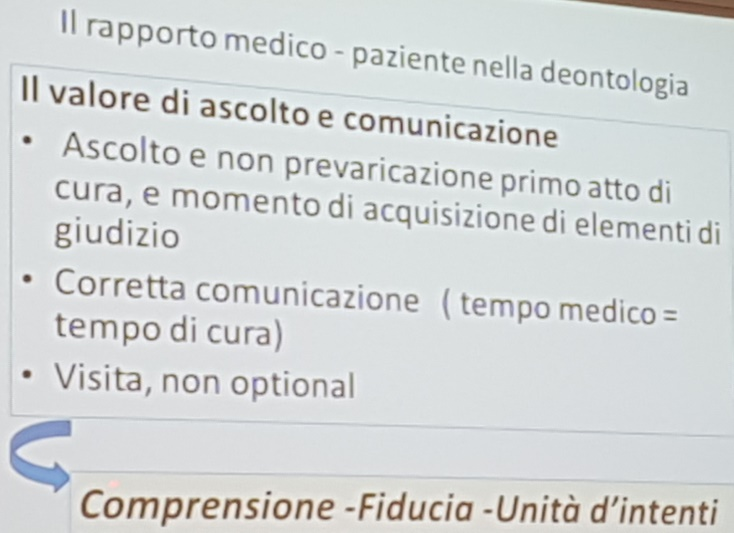
\includegraphics[width=5.10229in,height=4.41667in]{media/image6.jpeg}

GLI OSTACOLI ALL'ADERENZA (sotto-sottosezione)

Ci può essere scarsa \textbf{comunicazione medico paziente}:

\begin{itemize}
\item
  il paziente non conosce la sua malattia
\item
  il paziente non conosce i rischi e benefici della terapia
\item
  il paziente non conosce il corretto uso del farmaco
\item
  il medico prescrive un terapia troppo complessa
\end{itemize}

In questa situazione il paziente non ha colpe, sta al medico soddisfare
il bisogno di conoscenza del paziente. All'inizio della terapia bisogna
dedicare del tempo al paziente per illustrare la terapia, non è tempo
perso ma è tempo che si guadagna con la comprensione del problema.

Esempio: si riporta uno studio su 50 pazienti dimessi da un reparto di
medicina interna:

\begin{itemize}
\item
  i pazienti \textless{} 65 anni non conoscono il significato del 60\%
  dei farmaci prescritti;
\item
  i pazienti \textgreater{} 65 non conoscono il significato dell'80\%
  dei farmaci prescritti;
\item
  solo al 28\% dei pazienti è stato spiegato (all'atto della dimissione
  e nel periodo di transizione compreso tra la dimissione dall'ospedale
  e la presa in carico dal medico del territorio) quali farmaci assumere
  e perché assumerli nonostante l'80\% dei pazienti riferisca che questo
  aumenterebbe la soddisfazione della cura sanitaria: il paziente si
  aspetta che gli venga spiegato perché assumere i farmaci prescritti.
  La lettera di dimissione (nella parte inerente alla terapia) deve
  essere letta al paziente, il paziente dimesso deve aver capito perché
  assumere la terapia. La terapia poi verrà ripresa e spiegata dal
  medico curante, ma potrebbero trascorrere giorni dalla dimissione
  prima che il paziente si rechi dal curante.
\end{itemize}

Da considerare anche \textbf{l'interazione paziente - Sistema
Sanitario}:

\begin{itemize}
\item
  non corretto accesso al luogo di cura (esempio appuntamenti non
  rispettati);
\item
  erogazione della terapia non ottimale da parte dello staff clinico (il
  messaggio espresso dal medico viene diluito dal team sanitario tanto
  da non essere idoneo);
\item
  difficoltà a reperire farmaci;
\item
  continue variazioni della terapia (da parte degli specialisti che non
  si rendono conto che questo sconcerta il paziente che finisce per non
  aderire alla terapia);
\item
  incapacità del paziente a raggiungere la farmacia (esistono pazienti
  che risparmiano i farmaci: se il farmaco deve essere assunto ogni
  giorno, loro lo assumono a giorni alterni così da temporeggiare finché
  qualcuno --il figlio-- non vada ad acquistare il farmaco; qualche
  lodevole farmacia si è posta il problema ma di fatto non esistono
  servizi a domicilio per la consegna dei farmaci agli anziani che sono
  impossibilitati a recarsi in farmacia)
\item
  farmaci ad alto costo e o farmaci non rimborsabili
\end{itemize}

Infine consideriamo l'\textbf{interazione medico - Sistema Sanitario}:

\begin{itemize}
\item
  scarsa conoscenza del formulario terapeutico (bisogna ammetterlo, a
  volte non siamo al passo con i nuovi farmaci)
\item
  scarsa conoscenza del costo dei farmaci
\item
  poca soddisfazione nel proprio lavoro
\item
  scarsa conoscenza delle linee guida
\item
  inappropriatezza prescrittiva
\end{itemize}

LA NECESSITÀ DI COINVOLGERE IL PAZIENTE (sotto-sottosezione)

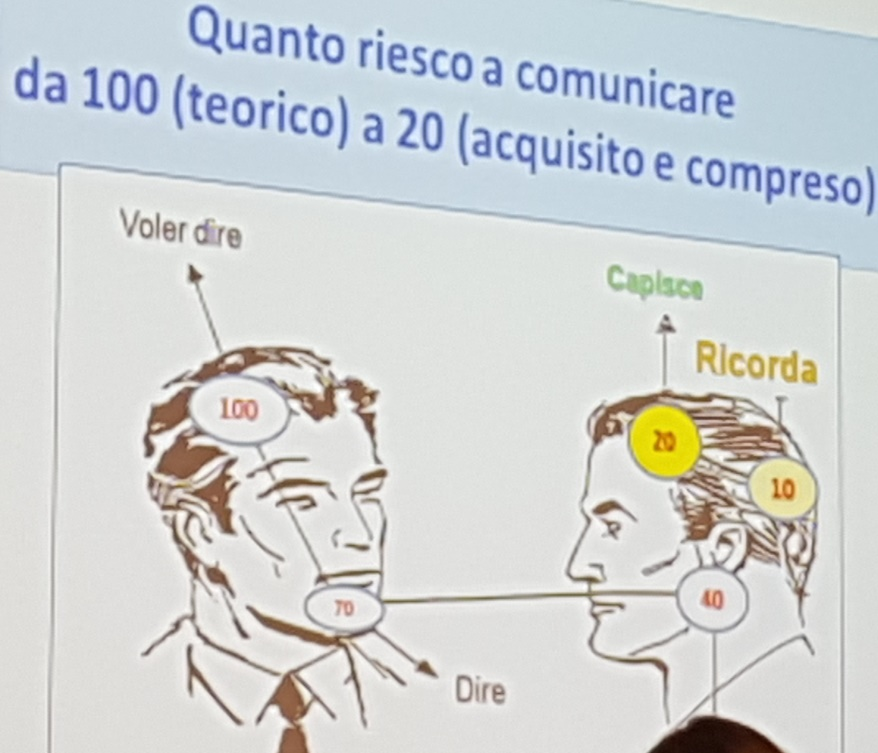
\includegraphics[width=6.03006in,height=3.55208in]{media/image7.jpeg}

Un approccio incentrato interamente sul medico comporta una elevata
probabilità di non aderenza. Un approccio incentrato sul paziente
facilita l'identificazione e la gestione delle condizioni di rischio.
Una migliore comunicazione (surrogato di empatia) migliora l'aderenza,
la soddisfazione e la prognosi clinica.

Esempi di migliore aderenza:

\begin{itemize}
\item
  nella terapia della depressione (Bauer et al. 2016)
\item
  nella terapia delle malattie reumatiche (Van Den Bemt et al. 2012)
\item
  nella terapia dell'infezione da HIV (Flickinger et al. 2016)
\item
  nella disassuefazione da fumo di tabacco (Champassac et al. 2014)
\end{itemize}

Linee guida NICE, 2016 (raccomandazioni sulla gestione della
multi-morbidità):

\emph{``Offri a tutti i pazienti l'opportunità di essere coinvolti nelle
decisioni che riguardano i farmaci da assumere. Cerca di capire in che
misura il paziente desidera essere coinvolto piuttosto che assumerlo a
priori.''}

CASO CLINICO (sottosezione)

In ambulatorio:

La signora A. nonostante i suoi 75 anni è una signora piacente. In
gioventù aveva ``fatto atletica'', come lei stessa ama ricordare. Ma non
ama le medicine. La signora ha una ipertensione sistolica ed alcuni anni
prima aveva presentato un TIA. La sua terapia comprende ACE + diuretico
ed ASA (aspirina). I valori pressori tuttavia non sono ben controllati e
il medico propone di aggiungere un calcio antagonista. La signora è
recalcitrante ma alla fine accetta. Passano alcune settimane e la
signora torna in ambulatorio. La pressione sistolica ora è ben
controllata ma la signora lamenta edemi malleolari soprattutto alla
sera. Sostiene con forza che per lei è un problema importante. Il
medico, dopo aver accertato la presenza di un modesto edema, e
considerando l'affollamento dell'ambulatorio, taglia corto, ribadisce
l'importanza della terapia e reitera la prescrizione dello stesso schema
terapeutico. Dopo un mese il medico apprende che la signora A. è stata
ricoverata per un ictus secondario a crisi ipertensiva. L'esame delle
confezioni dei farmaci rivela che la signora ha assunto irregolarmente
la terapia.

Quali possono essere stati i motivi della non aderenza alla terapia?

\begin{itemize}
\item
  insufficiente comunicazione medico -- paziente sugli effetti
  collaterali del farmaco;
\item
  scarsa consapevolezza da parte della paziente della condizione di
  rischio;
\item
  scarsa empatia medico paziente: i pazienti non sono tutti uguali, la
  signora A viene descritta come piacente nonostante l'età. L'effetto
  collaterale tollerabile per un altro paziente non è tollerato dalla
  signora A.
\end{itemize}

``Signora lei ha il 30\% di probabilità di avere le gambe un po' gonfie
alla sera, non si preoccupi, non vuol dire niente dal punto di vista
medico, se però questo assume una dimensione notevole o lei ne è
infastidita ritorni.'' Questo sarebbe potuto essere il messaggio.

EMPATIA E MALATTIE CRONICHE (sottosezione)

\emph{Academic Medicine (2012): The relationship between physician
empathy and disease complicantios: an empirical study of primary care
physician and their diabetic patients in Parma, Italy}

Questo lavoro ha destato molto interesse, è stato ripreso dai media
americani e italiani perché primo nel suo genere, inedito. Questo lavoro
è stato condotto dalla Jefferson University (Hojat) in collaborazione
con l'AUSL di Parma. Questo lavoro dimostra come l'empatia venga ad
incidere sulle complicanze acute di una patologia cronica quale il
diabete mellito. Lo strumento utilizzato è la Jeffersoy Empathy Scale,
scala somministrata a 242 medici dell'AUSL di Parma, tramite questa
scala si inquadra il livello di empatia dei medici.


\includegraphics[width=4.83333in,height=2.99683in]{media/image8.jpeg}

I medici sono stati divisi in tre livelli di empatia (alta, moderata,
bassa) e i livelli di empatia sono stati messi in correlazione con le
complicanze più gravi della malattia.

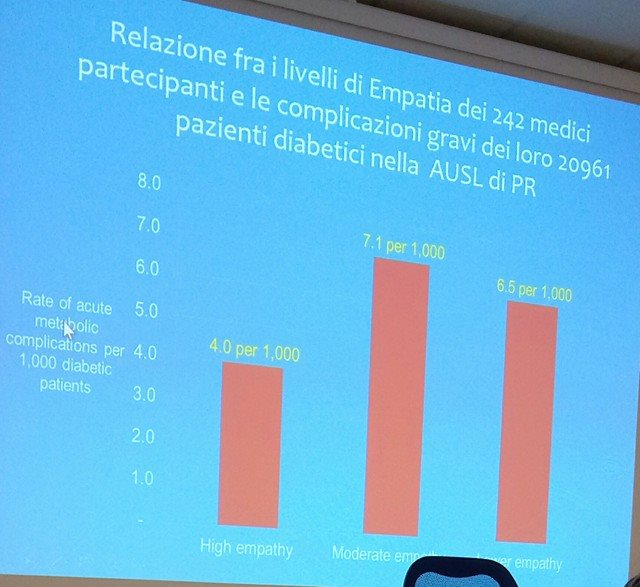
\includegraphics[width=6.66667in,height=3.61458in]{media/image9.jpeg}

Emergono due dati: 1) il numero di complicanze nei pazienti in cura
presso medici ``ad alta empatia'' è minore rispetto a quelle nei
pazienti seguite da medici ``a moderata empatia''; 2) non c'è differenza
tra il numero di complicanze nei pazienti in cura presso medici ``a
moderata empatia'' e ``bassa empatia'', la moderata empatia non è
sufficiente.

Quindi in conclusione l'empatia del medico:

a) è associata in modo statisticamente significativo all'outcome;

b) deve essere considerata come un elemento importante delle sue
competenze;

c) dovrebbe essere quindi valorizzata nella formazione del futuro
medico.

INSEGNARE E INCENTIVARE L'EMPATIA (sottosezione)

L'empatia può essere insegnata nell'ambito della nostra professione. Se
siamo convinti che l'empatia medico-paziente sia un requisito importante
del processo di cura e possa contribuire al raggiungimento di misurabili
outcome clinici perché non insegnarla durante il corso di studi medici e
delle professioni sanitarie con modelli congiunti? E continuare a
rinnovare queste competenze durante l'attività professionale con
attività di educazione continua (ECM)?

\emph{``L'empatia medico paziente declina col tempo sia durante gli
studi medici sia nel corso delle attività professionali.''}

Neumann

\emph{``Con il declino dell'empatia viene meno uno dei tre pilastri che
sorreggono la professionalità medica (conoscenza, capacità procedurali
ed empatia).''}

Novack

Dobbiamo conoscere quali sono gli ostacoli all'empatia medico-paziente:

\begin{itemize}
\item
  diminuzione del tempo dedicato al paziente;
\end{itemize}

\begin{itemize}
\item
  sistema sanitario orientato verso criteri economici (farmaco-economia,
  dott. Knock);
\item
  indebolimento della figura e del ruolo del medico;
\item
  figura del medico rappresentata (dai media che negli incidenti danno
  per scontato che la colpa sia dei medici) e percepita come egoistica,
  non etica e non autonoma;
\item
  fiducia eccessiva nella tecnologia (esempio: faccio l'eco ma non palpo
  il fegato);
\item
  medicina difensiva
\end{itemize}

Quindi come possiamo fare ad insegnare e ad incentivare l'empatia?
Tratto da un libro di Hojat:

\begin{itemize}
\item
  migliorare le capacità di relazioni interpersonali
\item
  analisi delle registrazioni audio video degli incontri con pazienti
\item
  proporre modelli di ruolo con simulazioni (che vengono analizzati
  insieme ai prof.)
\item
  valorizzare le esperienze del paziente in ospedale o in altri luoghi
  di cura
\item
  migliorare le capacità narrative degli operatori sanitari: importanza
  della narrazione (siamo capaci di narrare le malattie e le decisioni
  terapeutiche ai pazienti?)
\item
  incorporare lo studio della letteratura nel curriculum di studi
  (letteratura consigliata dai prof., storie inerenti la professione
  medica)
\item
  metodo Balint
\end{itemize}

\emph{``È importante conoscere che tipo di persona ha una determinata
malattia nello stesso modo con cui si cerca di conoscere quale tipo di
malattia abbia quella persona''.}

William Osler

\end{document}
